\chapter{Julia-Mengen}
\rhead{Julia-Mengen}
\begin{refsection}

\chapterauthor{Andreas M"uller}
\section{Dynamische Systeme und Iteration}
In der Analyis lernt man "uber 
gew"ohnliche Differentialgleichung, dass L"osungen f"ur eine gewisse
Zeit existieren und eindeutig seien.
Nur gerade f"ur lineare Differentialgleichungen lassen sich Aussagen 
dar"uber machen, ob f"ur lange Zeit L"osungen existieren.
Die elementare Theorie ist im wesentlichen eine lokale.
In den Anwendungen werden nicht lineare Differentialgleichungen immer
wichtiger.
Solche Probleme lassen sich manchmal linearisieren, womit ausreichend
genaue Aussagen erhalten werden k"onnen.
Ist jedoch die Nichtlinearit"at ausgepr"agt genug, darf sie nicht l"anger
vernachl"assigt werden.
Mit einer analytischen L"osung einer nichtlinearen Differentialgleichung
kann man nur in Ausnahmef"allen rechnen, dies ist aber meist auch nicht
n"otig. Oft reicht es, qualitative Aussagen "uber das Verhalten der
L"osung zu haben,
insbesondere die Stabilit"at nichtlinearer Systeme "uber lange Zeit.
Die Theorie der dynamischen Systeme macht allgemeine Aussagen "uber das
Verhalten von L"osungen von Differentialgleichungen auch "uber grosse
Zeitintervalle.

Wir betrachten ein dynamisches System, beschrieben durch eine
gew"ohnliche Differentialgleichung $\dot x= f(t,x)$, welches eine
periodische Bahn ausgehend vom Startwert $x_0$ hat.
Ist $T$ die Bahnperiode, gilt also
$x(nT)=x_0$ f"ur $n\in\mathbb N$.
Die Theorie der dynamischen Systeme interessiert sich f"ur das Verhalten
der L"osung bei einer kleinen "Anderung von $x_0$.

Man betrachte jetzt eine Ebene $H$ senkrecht auf die Bahnkurve im Punkt $x_0$.
Bahnen, die von einem Punkt in $H$ gen"ugend nahe bei $x_0$ ausgehen, werden
nach ungef"ahr der Zeit $T$ wieder in der N"ahe von $x_0$ durch $H$ gehen.
Man kann also zu jedem Startpunkt $x\in H$ nahe bei $x_0$ den ersten
Durchstosspunkt $g(x)$ der Bahn durch $H$ finden.
Die Abbildung $x\mapsto g(x)$ enth"alt die gleiche Information "uber das
Verhalten von L"osungen in der N"ahe von $x_0$ wie die urspr"ungliche
Differentialgleichung.
Dies zeigt, dass es reicht, das Verhalten von nichtlinearen Abbildungen
unter Iteration zu verstehen.

Die einfachste nichtlineare Abbildung in einer Dimension ist
die sogenannte logistische Abbildung \cite{julia:logistic}
\[
f_a(x)=ax(1-x).
\]
Wir untersuchen Iterationsfolgen $x_{n+1}=f_a(x_n)$ der logistischen Abbildung
ausgehend von Startpunkten in $[0,1]$.
Die Funktion hat einen Fixpunk $f_a(0)=0$, und f"ur $a < 1$ f"uhren Iterationen
immer wieder zum Punkt $0$ zur"uck.
Sobald $a>1$ wird, "andert sich dieses Verhalten.
Zun"achst tritt ein einzelner Fixpunkt bei $x=\frac{1-a}a$ auf.
Dieser Fixpunkt wird bei $a=3$ instabil und spaltet sich einen Zyklus 
mit Periode zwei auf.
Mit zunehmendem $a$ spaltet sich der Zyklus erneut auf, er durchl"auft
eine Kaskade von Periodenverdoppelungen
(Abbildung~\ref{julia:periodenverdoppelung}).
\begin{figure}
\begin{center}
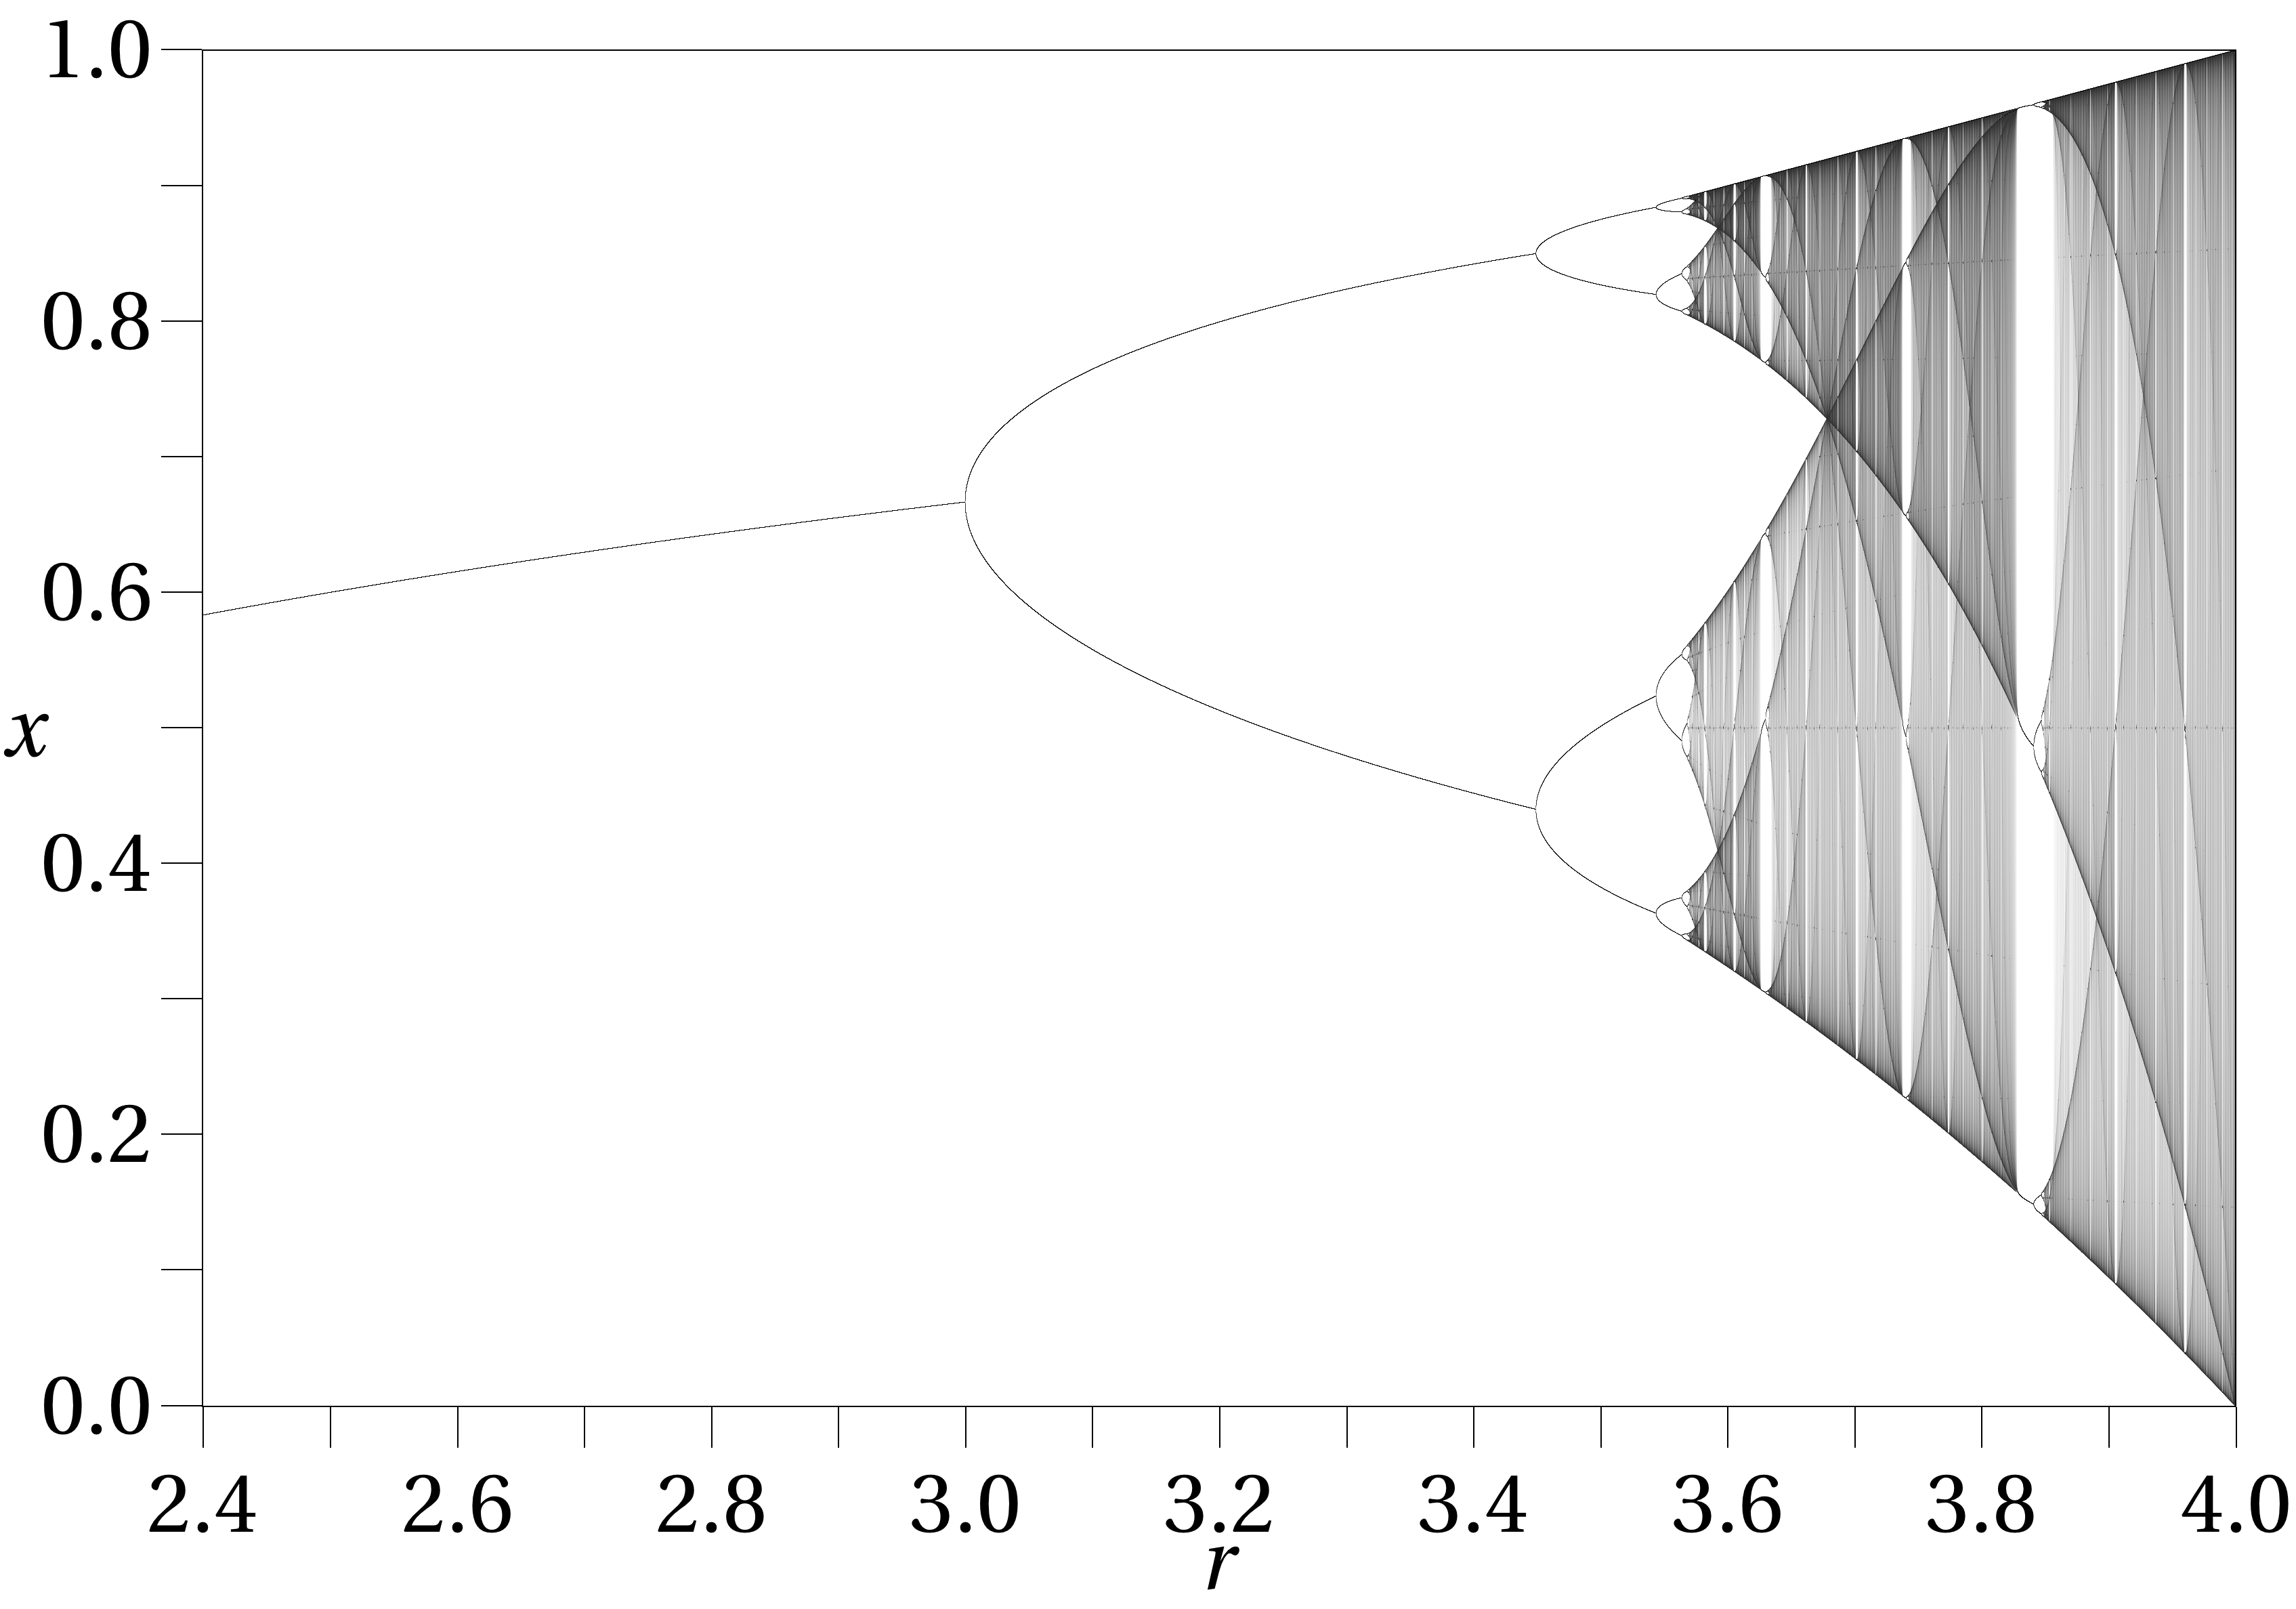
\includegraphics[width=0.7\hsize]{julia/logistic.png}
\end{center}
\caption{Periodenverdoppelungen bei der logistischen Abbildung in
Abh"angigkeit vom Parameter (aus \cite{julia:logistic}).
\label{julia:periodenverdoppelung}}
\end{figure}

Das bei der logistischen Abbildung beobachtete Verhalten tritt auch in
anderen Beispielen auf, zum Beispiel konnte es bei einem nichtlinearen
Halbleiter-Oszillator beobachtet werden.
In der Praxis h"angen Systeme meist von mehreren Parametern ab, es liegt
also nahe zu fragen, wie die Gebiete im Parameterraum aussehen, f"ur
die die Iteration einer nichtlinearen, von einem Parameter $a\in\mathbb R^n$
abh"angige Funktion konvergiert oder divergiert.

Ein besonders interessanter Spezialfall ist die einfachste nichtlineare
Funktion in den komplexen Zahlen, die Abbildung
\[
f_c(z)=z^2 + c,\qquad z,c\in\mathbb C,
\]
sie ist die direkte Verallgemeinerung der logistischen Abbildung auf
komplexe Zahlen.
Gaston Julia und Pierre Fatou haben die Iterationen rationaler 
Funktionen komplexer Variablen bereits zu Beginn des zwanzigsten
Jahrhunderts studiert, ohne allerdings den Luxus moderner Computergraphik
zur Verf"ugung zu haben. Sie haben sich speziell f"ur die Menge der
Startwerte interessiert, die zu einem bestimmten Verhalten der
Iterierten f"uhrt.

Verwandt mit der Frage nach der Menge der Startwerte, die zu einem
bestimmten Verhalten f"uhren, ist die Frage nach der Menge der Parameter,
die zu einem bestimmten Verhalten f"uhren.
Die Menge der Punkte $c\in\mathbb C$, f"ur die die Iterierten der
Funktion $f_c(z)$ mit Startwert $0$ beschr"ankt bleiben, heisst die
Mandelbrot-Menge, auch als ``Apfelm"annchen'' bekannt.

\section{Was sind Julia-Mengen?}
F"ur jede komplexe Zahl $c\in\mathbb C$ kann man die Iterationen der
Funktion
\begin{equation}
f_c(z)=z^2 + c
\label{julia:quadratic}
\end{equation}
untersuchen.
Ausgehend von einem Anfangswert $z_0\in\mathbb C$ bilden wir die Folge
\[
z_1=f(z_0),\;z_2=f(z_1),\;z_3=f(z_2)\;\dots, z_{n+1}=f(z_n),\;\dots
\]
F"ur $|z|\ge |c|$ und $|z|\ge 3$ folgt
\[
|f_c(z)|= |z^2+c|\ge |z|^2-|c|\ge |z|^2-|z|=|z|(|z|-1)\ge |z|\ge 2|z|.
\]
Die Iterierten von $z_n$ wachsen exponentiell schnell "uber alle Grenzen.

Es ist aber auch m"oglich, dass f"ur einzelne Punkte die Folge $z_n$ 
beschr"ankt bleiben. Im besten Fall werden sie gegen einen Punkt
$\hat z$ konvergieren.
Der Punkt $\hat z$ ist ein Fixpunkt von $f_c$, denn
\[
\hat z = \lim_{n\to \infty}f_c^{n}(z)\quad\Rightarrow\quad
f_c(\hat z)=f_c(\lim_{n\to\infty}f_c^n(z))=\lim_{n\to\infty}f_c^{n+1}(z)=\hat z.
\]
Die Folge $z_n$ muss aber nicht unbedingt gegen einen Punkt konvergieren,
es kann auch einen Zyklus von $k$ Punkten $\hat z_1,\dots,\hat z_k$ geben
so, dass
\[
z_{kn+1}\to \hat z_1,\quad
z_{kn+2}\to \hat z_2,\quad
z_{kn+3}\to \hat z_3,\quad\dots,\quad
z_{kn+k}\to \hat z_k.
\]

Die komplexe Ebene besteht also aus h"ochstens zwei Regionen: dem Bereich
von komplexen Zahlen, die bei Iteration "uber alle Grenzen wachsen, und
einem Bereich von Punkten, die bei Iteration gegen einen Zyklus konvergieren.
Dazwischen gibt es eine Menge von Punkten, f"ur den die Iterationen weder
zum einen noch zum anderen Verhalten f"uhren.
Auf dieser Menge ist die Iteration chaotisch, sie
heisst die Julia-Menge von $f_c$.

\begin{beispiel}
Im Fall $c=0$ ist $f_0(z)=z^2$. Da jede komplexe Zahl geschrieben werden
kann als $z=re^{i\varphi}$, sind die Iterierten von $f_0$:
\[
z_1=r^2e^{2i\varphi},
z_2=r^4e^{4i\varphi},
z_3=r^8e^{8i\varphi},
z_4=r^{16}e^{16i\varphi},\dots,
z_n=r^{2^n}e^{2^ni\varphi},\dots
\]
Wenn $r < 1$ ist, dann werden die Iterierten $z_n$ immer kleiner, die
Folge konvergiert gegen $0$.
Falls $r>1$ dann wachsen die Iterierten "uber alle Grenzen.
Im Falle $r=1$ bleiben die Iterierten auf dem Einheitskreis.
Die komplexe Ebene wird also in drei Bereiche geteilt: das
Innere des Einheitskreises besteht aus Zahlen, deren Iterierte gegen
0 konvergieren, das "Aussere des Einheitskreises besteht aus Zahlen,
deren Iterierte gegen $\infty$ konvergieren.
Die Grenze zwischen den beiden Bereichen ist der Einheitskreis selber,
die Iterierten der Zahlen auf dem Einheitskreis konvergieren im
allgemeinen nicht.

Der Einheitskreis ist die Julia-Menge der Abbildung $f_c$ f"ur $c=0$.
\end{beispiel}

F"ur Werte $c\ne 0$ des Parameters kann die Julia-Menge sehr kompliziert
werden, so kompliziert, dass sie nur dank Computer-Berechnungen
ausreichend detailliert visualisiert werden kann.

Die Iteration der quadratischen Abbildungen (\ref{julia:quadratic})
wurden sorgf"altig studiert, sie sind relativ einfach, zeigen aber
trotzdem viele Eigenschaften der nichtlinearen dynamischen Systeme.
Insbesondere zeigt schon $f_0$ auf dem Einheitskreis chaotisches
Verhalten \cite{julia:devaney}.

Die Julia-Mengen werden derart kompliziert, dass man ihnen keine ganzzahlige
Dimension mehr zuweisen kann. Vergr"ossert man einen Ausschnitt, werden
immer mehr Details sichtbar, die ``Kurve'' wird immer komplizierter.
Ist ist oft m"oglich, den Julia-Mengen eine gebrochenzahlen Dimension
zuzuweisen.
Die Definition dieser gebrochenzahligen Dimensionen ist nicht ganz
selbstverst"andlich, Mengen mit gebrochenzahliger Dimension treten
aber mindestens n"aherungsweise in der Natur immer wieder auf, sie
sind auch als Fraktale bekannt \cite{julia:falconer}.

In den Abbildungen~\ref{julia:a} bis \ref{julia:h} sind Julia-Mengen
f"ur eine Auswahl von Parameterwerten $c$ visualisiert.
F"ur \ref{julia:a} bis \ref{julia:f} gibt es jeweils einen Zyklus, gegen
den ein Teil der Iterationsfolgen konvergiert.
In \ref{julia:g} und \ref{julia:h} ist die Menge der Startpunkte, die zu einem
Zyklus f"uhren auf die leere Menge zusammengeschrumpft, es bleibt nur
noch die Julia-Menge "ubrig, bestehend aus Startwerten, die nicht zu
Iterationen gegen $\infty$ f"uhren.
In \ref{julia:g} zerf"allt die Julia-Menge in einzelne Punkte, 
man spricht auch von ``Cantor-Staub'',
in \ref{julia:h} besteht sie aus einem fraktalen Baum.

\section{Berechnung von Julia-Mengen}
Es gibt zwei M"oglichkeiten, eine Julia-Menge sichtbar zu machen.
In den F"allen, wo ein Fixpunkt $\hat z$ existiert, kann man f"ur jeden
Punkt der komplexen Ebene die Iterationsfolge $z_n$ berechnen, und
entscheiden ob sie gegen $\infty$ oder einen Zyklus konvergiert.
Die Julia-Menge ist dann die Grenze zwischen diesen Bereichen.

Dies funktioniert allerdings nicht f"ur Parameterwerte, f"ur die
es keinen Zyklus gibt, gegen den die Folge $z_n$ konvergieren k"onnte.
In diesem Fall kann man die Abbildung $f_c(z)$ umkehren: wenn die
Punkte $z_n$ von der Julia-Menge weg gegen $\infty$ konvergieren, dann 
m"ussen die Urbilder gegen die Juliamenge konvergieren.
Man kann also die Julia-Menge dadurch finden, dass man alle Urbilder
bestimmt.

\subsection{Julia-Mengen durch Iteration}
Um ein Bild der Julia-Menge zum Parameter $c$ zu erhalten, berechnet
man f"ur jeden Startpunkt $z_0\in\mathbb C$ die Folge $z_n$ und
bestimmt den kleinsten Wert $n$, f"ur den $|z_n|>b$ ist, wobei $b$
irgend eine fest Schranke ist.
Der Pixel zum Punkt $z_0$ wird mit einer Farbe eingef"arbt, die von $n$
abh"angt.
Falls $z_n$ die Grenze $b$ nicht "uberschreitet, bleibt der Pixel schwarz.

Die Berechnung der Iterationsfolge ist f"ur jeden Pixel vollkommen
unabh"angig von jedem anderen Pixel, dieses Beispiel ist als pr"adestiniert
f"ur die Berechnung mit OpenCL.
Jeder Pixel stellt ein eigenes Work-Item dar.
Das Programm {\tt julia1.c} im Repository implementiert diese Strategie.

Diese Methode zeigt nicht die Julia-Menge, sondern die Menge der Startpunkte,
die unter Iteration nach $\infty$ konvergieren. Den Bereichen von Startpunkten,
die zu beschr"ankten Iterationsfolgen f"uhren, kann mit dieser Methode
keine Farbe zugeordnet werden.
In den Abbildungen~\ref{julia:a} bis \ref{julia:h} sind diese Bereiche 
schwarz dargestellt.
Die Julia-Menge ist also der Rand des schwarzen Gebietes.

F"ur gewisse Parameter, zum Beispiel f"ur $c=i$ (Abbildung~\ref{julia:g})
oder $c=0.66i$ (Abbildung~\ref{julia:h}), enth"alt die ``schwarze'' Menge
keine inneren Punkte mehr, man kann sie daher auf den Bildern
kaum mehr erkennen.
In diesen F"allen ist die Julia-Menge nur daran erkennbar, dass Startwerte
nahe der Julia-Menge viele Iterationen ben"otigen, bis $z_n$ "uber die
gew"ahlte Schranke gewachsen ist.

Zusammenfassend kann man f"ur diese Methode folgende Eigenarten der
Implementation festhalten:
\begin{itemize}
\item Jeder Pixel ist ein Work-Item. Dimensionen des Resultat Array
ergeben sich somit aus der globalen Gr"osse.
\item Der Startwert $c$, der einem Work-Item entspricht, kann mit Hilfe
weniger, in einem globalen Array "ubergebener Parameter, aus der
ID des Work-Item errechnet werden.
\item Die Resultate werden in einem Array zur"uckgegeben, in dem jedes
Work-Item genau einen Wert speichert, die Anzahl der Iterationen bis
zum Erreichen der Schranke.
Eine Initialisierung des Array ist nicht n"otig.
\end{itemize}

\subsection{Julia-Mengen durch Inverse Iteration}
Die hier beschriebene Methode zur Berechnung von Julia-Mengen wird in
\cite{julia:peitgenrichter} als Inverse Iteration Method bezeichnet.
F"ur die meisten Startpunkte konvergiert die Iterationen der Abbildung
$z\mapsto f_c(z)$ konvergiert gegen $\infty$
oder einen Zyklus, insbesondere entfernen sich die Punkte $z_n$ von der
Julia-Menge.
Verfolgt man die Iteration r"uckw"arts, also indem man eine Folge
$\tilde z_{n+1}=f_c^{-1}(\tilde z_n)$ konstruiert, dann n"ahern sich die
Punkte der Julia-Menge. Indem man die Punkte $\tilde z_n$ f"ur grosse $n$
plottet, erh"alt man eine Apprxomation der Julia-Menge.

Die Konstruktion der Folge $\tilde z_n$ ist nicht eindeugt, denn die
Gleichung
\[
z_n= f_c(z_{n+1})=\tilde z_{n+1}^2+c
\]
hat zwei L"osungen $\pm\sqrt{z_n-c}$. 
Um eine m"oglichst gute Approximation der Julia-Menge zu bekommen, 
werden wir jede m"ogliche Wurzel r"uckw"arts verfolgen wollen.
Die zwei Urbilder von $z$ haben unter $f_c$ insgesamt vier Urbilder, 
die wiederum haben acht Urbilder.
Jede weitere Iteration verdoppelt die Anzahl der Urbilder, daf"ur ist
in OpenCL kein Platz vorhanden, wir k"onnen nun mal in OpenCL nicht beliebig
Speicher allozieren.

Wir verwenden daher eine andere Strategie: wir w"ahlen jeweils nur eines
der Urbilder, wobei wir die Auswahl mit Hilfe von Zufallszahlen steuern.
Diese Berechnung wiederholen wir viele Male, jeweils mit einer anderen
Zufallszahlfolge.
Auf diese Weise werden ebenfalls alle Punkte der Julia-Menge irgendwann
approximiert.

Mit dieser Strategie handeln wir uns aber ein neues Problem ein: wir brauchen
eine Folge von Zufallszahlen.
OpenCL stellt kein API f"ur Zufallszahlen zur Verf"ugung, dies muss also
ebenfalls im OpenCL Code implementiert werden.
Die Anforderungen an die Qualit"at der Zufallszahlen ist nicht besonders
hoch, ein einfacher Zufallszahlgenerator auf der Basis von linearen
Kongruenzen wie der Lehmer-Generator \cite{julia:lehmer},
auch bekannt als Park-Miller Generator, reicht v"ollig aus.

Die inverse Iteration f"uhrt f"ur stark verzweigte Julia-Mengen nicht
zu guten Resultaten.
Man kann dies dank der fraktalen Natur der Julia-Menge verstehen.
Beginnt man mit einer geschlossenen Kurve $\gamma_0$ in $\mathbb C$,
dann sind die Urbilder $\gamma_{n+1} = f_c(\gamma_n)$ jeweils Vereinigungen
von geschlossenen Kurven, die die Julia-Menge immer besser Approximieren.
Wegen der fraktalen Natur der Julia-Menge wird $\gamma_{n}$ mit zunehmendem
$n$ immer l"anger.
Entsprechend wird die Dichte der durch Inverse Iteration
erzeugten Punkte auf $\gamma_{n+1}$ immer kleiner. 
F"ur Julia-Mengen, die sich wie Kurven verhalten, ist die Approximation
recht gut (Abbildungen~\ref{julia:a} und \ref{julia:h}).
Am anderen Ende des Spektrum befinden sich Julia-Mengen, die in Cantor-Staub
zerfallen wie in Abbildung~\ref{julia:g}, welche nur sehr schlechte
Approximationen haben.

Als Charakteristika dieser L"osung halten wir fest:
\begin{itemize}
\item Resultat ist ein Array von Pixel-Werten, in jedem Pixel wird
gez"ahlt, wie oft dieser Punkt in der inversen Iteration getroffen wurde.
\item Die Strukturierung der Work-Items ist willk"urlich.
\item Kein Bezug zwischen Work-Items und Pixeln, daher muss ein bereits
mit 0 initialisierter Array dem Kernel "ubergeben werden.
Initialisierung durch den Kernel und Synchronisation w"aren viel zu teuer.
\item
Zur optimalen Ausnutzung der
Hardware muss die m"ogliche Workgroup-Gr"osse abgefragt werden.
In diesem Fall ist sie wegen des umfangreicheren
Kernels deutlich kleiner als das Maximum.
\item
Zufallszahlen notwendig, erzeugung mit Hilfe des Park-Miller
Zufallszahl-Generators, initialisiert mit der Work-ID.
\end{itemize}

\begin{figure}
\begin{center}
\includegraphics[width=\hsize]{julia/c-a-low.png}

\bigskip

\includegraphics[width=\hsize]{julia/j-a-low.png}
\end{center}
\caption{Julia-Menge f"ur $c= -0.1+0.1i$\label{julia:a}}
\end{figure}

\begin{figure}
\begin{center}
\includegraphics[width=\hsize]{julia/c-b-low.png}

\bigskip

\includegraphics[width=\hsize]{julia/j-b-low.png}
\end{center}
\caption{Julia-Menge f"ur $c= -0.5+0.5i$\label{julia:b}}
\end{figure}

\begin{figure}
\begin{center}
\includegraphics[width=\hsize]{julia/c-c-low.png}

\bigskip

\includegraphics[width=\hsize]{julia/j-c-low.png}
\end{center}
\caption{Julia-Menge f"ur $c= -1+0.05i$\label{julia:c}}
\end{figure}

\begin{figure}
\begin{center}
\includegraphics[width=\hsize]{julia/c-d-low.png}

\bigskip

\includegraphics[width=\hsize]{julia/j-d-low.png}
\end{center}
\caption{Julia-Menge f"ur $c= -0.1+0.75i$\label{julia:d}}
\end{figure}

\begin{figure}
\begin{center}
\includegraphics[width=\hsize]{julia/c-e-low.png}

\bigskip

\includegraphics[width=\hsize]{julia/j-e-low.png}
\end{center}
\caption{Julia-Menge f"ur $c= 0.25+0.52i$\label{julia:e}}
\end{figure}

\begin{figure}
\begin{center}
\includegraphics[width=\hsize]{julia/c-f-low.png}

\bigskip

\includegraphics[width=\hsize]{julia/j-f-low.png}
\end{center}
\caption{Julia-Menge f"ur $c= -0.5+0.55i$\label{julia:f}}
\end{figure}

\begin{figure}
\begin{center}
\includegraphics[width=\hsize]{julia/c-g-low.png}

\bigskip

\includegraphics[width=\hsize]{julia/j-g-low.png}
\end{center}
\caption{Julia-Menge f"ur $c= 0.66i$\label{julia:g}}
\end{figure}

\begin{figure}
\begin{center}
\includegraphics[width=\hsize]{julia/c-h-low.png}

\bigskip

\includegraphics[width=\hsize]{julia/j-h-low.png}
\end{center}
\caption{Julia-Menge f"ur $c= -i$\label{julia:h}}
\end{figure}

\printbibliography[heading=subbibliography]
\end{refsection}
